\documentclass[tikz]{standalone}

\usepackage{mathtools}

\usetikzlibrary{calc,positioning}

\begin{document}
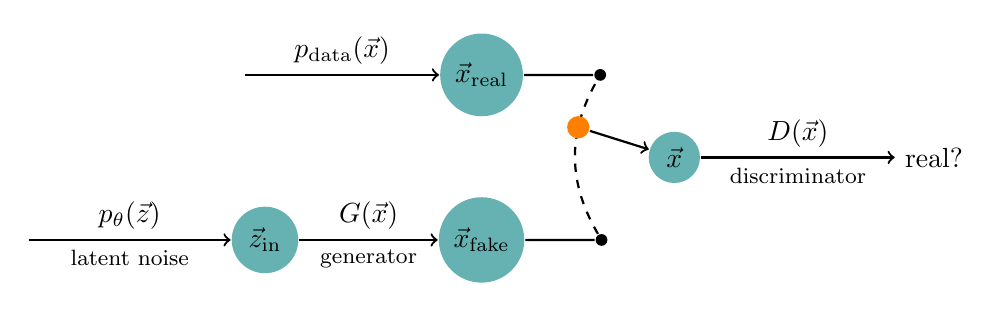
\begin{tikzpicture}[
    ->, thick,
    node/.style={circle, fill=teal!60},
    label/.style={below, font=\footnotesize},
  ]

  \node[node] (zin) {$\vec z_\text{in}$};
  \node[node, right=5em of zin] (fake) {$\vec x_\text{fake}$};
  \draw (zin) -- node[above] {$G(\vec x)$} node[label] {generator} (fake);

  \draw[<-] (zin) -- node[above] {$p_\theta(\vec z)$} node[label] {latent noise} ++(-3,0);
  \node[node, above=of fake] (real) {$\vec x_\text{real}$};
  \draw[<-] (real) -- node[above] {$p_\text{data}(\vec x)$} ++(-3,0);
  \node[node, right=6em of fake] (D) at ($(fake)!0.5!(real)$) {$\vec x$};
  \node[right=7em of D] (out) {real?};
  \draw (D) -- node[above] {$D(\vec x)$} node[label] {discriminator} (out);

  \coordinate[right=2.5em of fake, circle, fill, inner sep=0.15em] (pt1);
  \coordinate[right=2.5em of real, circle, fill, inner sep=0.15em] (pt2);

  \draw[-, dashed] (pt1) edge[bend left] coordinate[circle, fill=orange, inner sep=1mm, pos=0.7] (pt3) (pt2);
  \draw (fake) -- (pt1) (real) -- (pt2) (pt3) -- (D);

\end{tikzpicture}
\end{document}
